\section{Introduction and Fundamentals}
\frame{\tableofcontents[currentsection]}
	\subsection{Introduction}
	\begin{frame}
		\frametitle{Introduction}
		kurzes blabla
	\end{frame}
	\begin{frame}
		\frametitle{Flow Properties}
		\begin{itemize}
			\item Compressible flow
			\item Ideal gas 
			\begin{itemize}
				\item Heat capacity ratio $\gamma = \dfrac{c_p}{c_v} = 1.4$
			\end{itemize}
			\item Newtonian fluid
			\begin{itemize}
				\item Stress tensor $\tau_{ij} = \mu \left[\left(\dfrac{\partial u_i}{\partial x_j} + \dfrac{\partial u_j}{\partial x_i}\right)- \dfrac{2}{3}\dfrac{\partial u_k}{\partial x_k} \delta_{ij}\right]$
			\end{itemize}
			\item Mach number $\text{Ma} = \dfrac{v_\infty}{a_\infty} = 0.2$
			\item Reynolds number $\text{Re} = \dfrac{\rho_\infty V_\infty L}{\mu_\infty} \propto \dfrac{\text{inertia forces}}{\text{viscous forces}}$
			\item Prandtl number $\text{Pr} = \dfrac{ \mu_\infty c_p}{k_\infty} \propto \dfrac{\text{viscous diffusion rate}}{\text{thermal diffusion rate}}$
		\end{itemize}
	\end{frame}
	\begin{frame}
		\frametitle{Non-dimensional 2D Compressible Navier-Stokes Equations}

%		time discretisation durch Runge-Kutta erster Ordnung -> expliziter Euler
\vspace{-0.5cm}
\begin{itemize}
	\item 2D
	\item Non-dimensional conserved flow variables: density $\rho$, momentum $\rho u$, $\rho v$, energy $\rho E$
\end{itemize}
\vspace{-0.3cm}
	\scalebox{0.9}{
		\begin{minipage}{\the\textwidth}
		\begin{align*}
			\tcbhighmath[drop fuzzy shadow,colframe=myblue]{\dfrac{\partial U}{\partial t}}+\tcbhighmath[drop fuzzy shadow,colframe=mygreen]{ \left(\dfrac{\partial F_c^x(U)}{\partial x} + \dfrac{\partial F_c^y(U)}{\partial y}\right)} - \tcbhighmath[drop fuzzy shadow,colframe=myred]{\left( \dfrac{\partial F_v^x(U, \nabla U)}{\partial x} + \dfrac{\partial F_v^y(U, \nabla U}{\partial y}\right)} = 0 			
		\end{align*}
	\end{minipage}
	}
	\begin{columns}[t]
		\begin{column}{0.6\textwidth}
			%\column[t]{7cm}
			\scalebox{0.75}{
			\begin{minipage}{\the\textwidth}
			\begin{flalign*}
			U &=\left(\begin{array}{c} \rho\\	\rho u\\ \rho v\\ \rho E\\	\end{array} \right) \quad 
			F_c^x=\left(\begin{array}{c} \rho u\\	\rho u^2 +p\\ \rho u v\\ u(\rho E +p)\\	\end{array} \right) \quad 
			F_c^y=\left(\begin{array}{c} \rho v\\	\rho u v\\ \rho v^2 +p\\ v(\rho E +p)\\	\end{array} \right) \\[8pt]
			F_v^x &= \dfrac{1}{\text{Re}}\left(\begin{array}{c} 0\\	\tau_{xx}\\ \tau_{xy}\\ \tau_{xx} u + \tau_{xy} v + \dfrac{\gamma}{\text{Pr}(\gamma - 1)}\kappa\dfrac{\partial T}{\partial x}\\	\end{array} \right) \quad
			F_v^y = \dfrac{1}{\text{Re}}\left(\begin{array}{c} 0\\	\tau_{xy}\\ \tau_{yy}\\ \tau_{xy} u + \tau_{yy} v + \dfrac{\gamma}{\text{Pr}(\gamma - 1)}\kappa\dfrac{\partial T}{\partial y}\\	\end{array} \right)
			\end{flalign*}			
		\end{minipage}
	}
	\end{column}
	\begin{column}{0.35\textwidth}
		%	\column[t]{5cm}
	\vspace{-2cm}
	\begin{itemize}
		\bluedot Temporal derivative
		\greendot Convective fluxes
		\reddot Viscous fluxes
	\end{itemize}
\end{column}
\end{columns}

	\end{frame}
	\subsection{The Discontinuous Galerkin Method}
	\begin{frame}
		\frametitle{The Discontinuous Galerkin Space Discretisation}
		\begin{figure}
			\centering
			\subfloat[First order FEM \label{fig:a}]{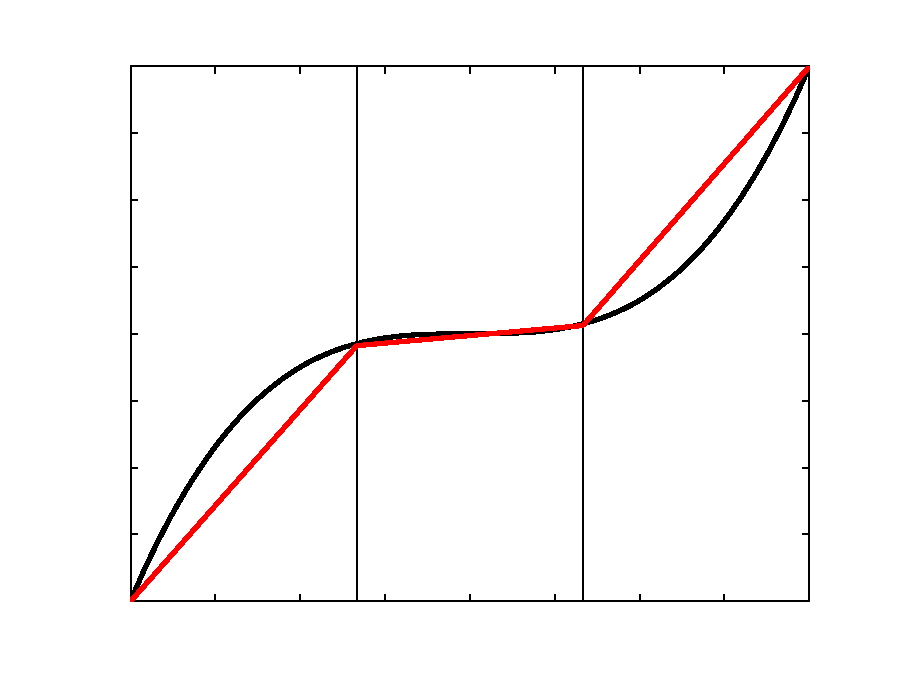
\includegraphics[width=0.28\textwidth]{img/fem.eps}}
			\subfloat[Zeroth order DG (FVM)\label{fig:b}]{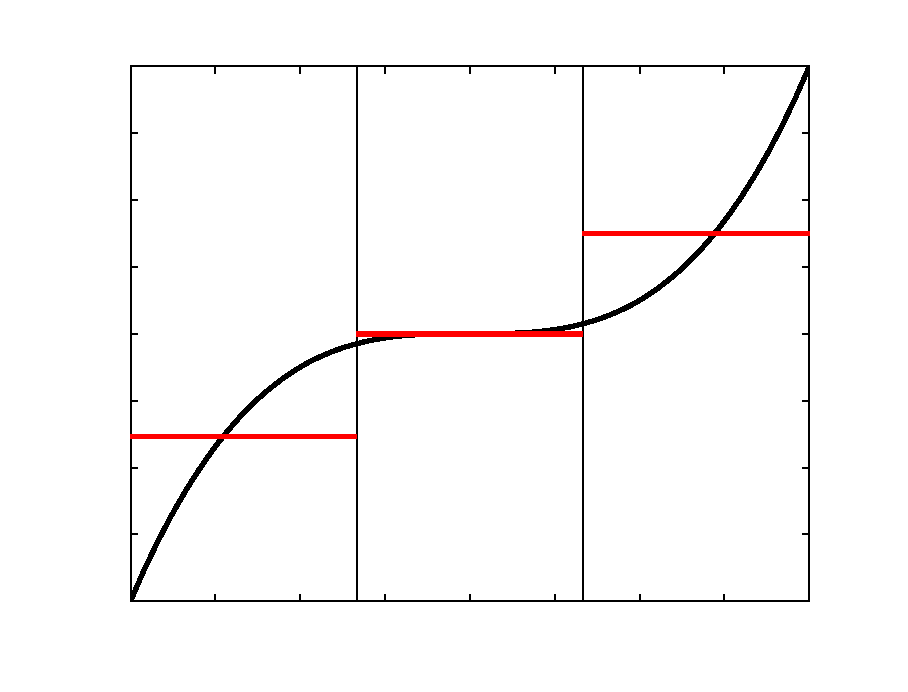
\includegraphics[width=0.28\textwidth]{img/fvm.eps}}
			\subfloat[First order DG \label{fig:c}]{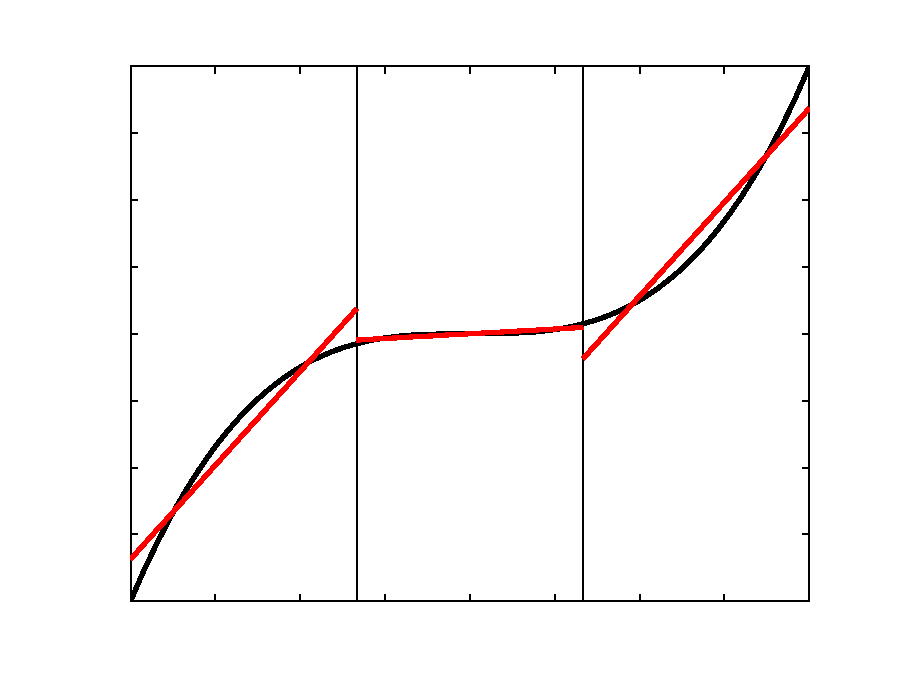
\includegraphics[width=0.28\textwidth]{img/dg.eps}}
			\caption{Comparison of FEM, FVM and DG}
			\label{fig:1}
		\end{figure}

		DG space discretisation Vorgehen, Bildchen, fluxes
	\end{frame}
	\subsection{The Immersed Boundary Method}
	\begin{frame}
		\frametitle{The Immersed Boundary Method}
		\begin{columns}[t]
			\column[]{7cm}
			\column[]{5cm}
			\begin{figure}[htbp]
				\vspace{-1cm}
				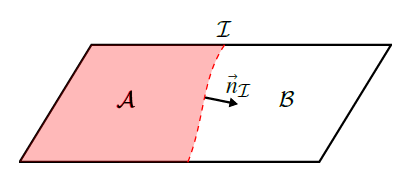
\includegraphics[width=\textwidth]{img/ibmcut.PNG}
				\caption{Cut cell with physical (red) and void region (white) [4]}\label{fig:cutcell}
			\end{figure} 
		\end{columns}
		regions mit Bild, Aufteilung Integrale
		mass matrix
		rk time discretisation formel
		cell agglomeration
	\end{frame}
	\begin{frame}
		\frametitle{Cell Agglomeration}
		\begin{columns}[t]
			\column[]{7cm}
			\column[]{5cm}
			\begin{figure}[htbp]
				\vspace{-1cm}
				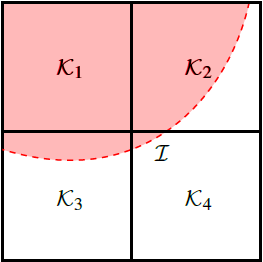
\includegraphics[height=0.3\textheight]{img/ibminitmesh.PNG}
				\caption*{(a) Initial mesh partitioning}
				\label{fig:init}
			\end{figure} 
			\begin{figure}[htbp]
				\vspace{-1cm}
				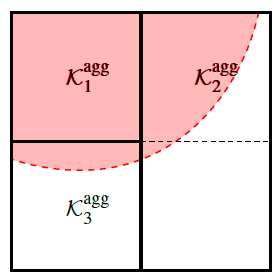
\includegraphics[height=0.3\textheight]{img/ibmagglomklein.PNG}
				\caption*{(b) Cell agglomeration with small agglomeration threshold}
				\label{fig:ineit}
			\end{figure} 
			\begin{figure}[htbp]
				\vspace{-1cm}
				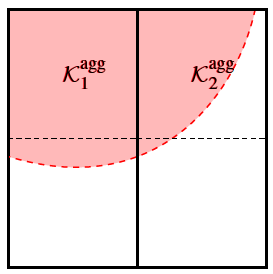
\includegraphics[height=0.3\textheight]{img/ibmagglomgross.PNG}
				\caption*{(c) Cell agglomeration with bigger agglomeration threshold}
				\label{fig:iwnit}
			\end{figure} 
		\end{columns}
		regions mit Bild, Aufteilung Integrale
		mass matrix
		rk time discretisation formel
		cell agglomeration
	\end{frame}